\documentclass[english]{article} 

\usepackage{geometry}

\usepackage{float}
\usepackage{xfrac}
\usepackage{mathrsfs} 
\usepackage{caption}
\usepackage{subcaption}
\usepackage[utf8]{inputenc}

\usepackage{amsmath}
\usepackage{amsfonts}
\usepackage{amssymb}
\usepackage{eurosym}
\usepackage{mathtools}
\usepackage{graphicx}
\usepackage{rotating}
\usepackage{setspace}
\usepackage{color}
\usepackage{fancyhdr}
\usepackage{ragged2e}
\usepackage{appendix}
\usepackage{tabularx}
\usepackage{multirow}
\usepackage{booktabs}
\usepackage{xfrac}
\usepackage{pgfplots}
\usepackage{url}
\usepackage{emptypage}
\usepackage{wrapfig}
\usepackage{dsfont}
\usepackage{soul}

\usepackage{csquotes}
\usepackage{hyperref}
%\usepackage{hyperref} %Ricordati di caricarlo alla fine
\pgfplotsset{compat=1.18}

\DeclareMathOperator{\diag}{diag}
\DeclareMathOperator{\dw}{d_w}
\DeclareMathOperator{\C}{C_{tc}}
\DeclareMathOperator{\T}{T}
\DeclareMathOperator{\MP}{MP}
\DeclareMathOperator{\KP}{KP}
\DeclareMathOperator{\K}{K}
\DeclareMathOperator{\Id}{Id}
\DeclareMathOperator{\SSpan}{Span}
%\DeclareMathOperator{\lim}{lim}
\DeclareMathOperator{\epi}{epi}


\newtheorem{example}{Example}
\newtheorem{assumption}{Assumption}
\newtheorem{definition}{Definition}
\newtheorem{theorem}{Theorem}
\newtheorem{corollary}{Corollary}[theorem]
\newtheorem{lemma}[theorem]{Lemma}
\newtheorem{prop}[theorem]{Proposition}
\newtheorem{observation}[theorem]{Observation}
\newtheorem{problem}{Problem}

\numberwithin{definition}{section}
\numberwithin{theorem}{section}
\numberwithin{problem}{section}

\newcommand{\nc}{\newcommand}
\nc{\boB}{{\mathbf{B}}}
\nc{\boL}{{\mathbf{L}}}
\nc{\boY}{{\mathbf{Y}}}
\nc{\boI}{{\mathbf{I}}}
\nc{\boV}{{\mathbf{V}}}
\nc{\boS}{{\mathbf{S}}}
\nc{\tV}{{\Tilde{{V}}}}
\nc{\tI}{{\Tilde{{I}}}}
\nc{\tY}{{\Tilde{{Y}}}}
\nc{\tS}{{\Tilde{{S}}}}
\nc{\fr}{{\rightarrow}}
\nc{\co}{{\nabla}}
\nc{\E}{\mathbb{E}}
\nc{\CG}{C_{\Sigma}^{\text{Gauss}}}
\nc{\var}{Var}
\nc{\pf}[1]{#1_{\#}} %push forward


\nc{\cu}{{\barline{\nabla}}}
\nc{\infint}{(-\infty,\infty]}


\nc{\sS}{ \mathscr{S}}
\nc{\sC}{ \mathscr{C}}
\nc{\cH}{{\mathcal H}}
\nc{\cR}{{\mathcal R}}
\nc{\cA}{{\mathcal A}}
\nc{\cG}{{\mathcal G}}
\nc{\cC}{{\mathcal C}}
\nc{\cD}{{\mathcal D}}
\nc{\cO}{{\mathcal O}}
\nc{\cI}{{\mathcal I}}
\nc{\cB}{{\mathcal B}}
\nc{\cY}{{\mathcal Y}}
\nc{\cK}{{\mathcal K}} 
\nc{\cX}{{\mathcal X}}
\nc{\cS}{{\mathcal S}}
\nc{\cE}{{\mathcal E}}
\nc{\cF}{{\mathcal F}}
\nc{\cZ}{{\mathcal Z}}
\nc{\cQ}{{\mathcal Q}}
\nc{\cP}{{\mathcal P}}
\nc{\cL}{{\mathcal L}}
\nc{\cM}{{\mathcal M}}
\nc{\cN}{{\mathcal N}}
\nc{\cT}{{\mathcal T}}
\nc{\cW}{{\mathcal W}}
\nc{\cU}{{\mathcal U}}
\nc{\cJ}{{\mathcal J}}
\nc{\cV}{{\mathcal V}}
\nc{\bH}{{\mathbb H}}
\nc{\bA}{{\mathbb A}}
\nc{\bG}{{\mathbb G}}
\nc{\bC}{{\mathbb C}}
\nc{\bO}{{\mathbb O}}
\nc{\bI}{{\mathbb I}}
\nc{\bB}{{\mathbb B}}
\nc{\bY}{{\mathbb Y}}
\nc{\bK}{{\mathbb K}} 
\nc{\bX}{{\mathbb X}}
\nc{\bS}{{\mathbb S}}
\nc{\bE}{{\mathbb E}}
\nc{\bF}{{\mathbb F}}
\nc{\bZ}{{\mathbb Z}}
\nc{\bQ}{{\mathbb Q}}
\nc{\bN}{{\mathbb N}}
\nc{\bP}{{\mathbb P}}
\nc{\bL}{{\mathbb L}}
\nc{\bM}{{\mathbb M}}
\nc{\bT}{{\mathbb T}}
\nc{\bW}{{\mathbb W}}
\nc{\bU}{{\mathbb U}}
\nc{\bD}{{\mathbb D}}
\nc{\bJ}{{\mathbb J}}
\nc{\bV}{{\mathbb V}}
\nc{\bR}{{\mathbb R}}


\newcommand{\virgolette}[1]{``#1''} %\virgolette{questo č fra virgolette}%
%\usepackage{frontespizio}
\newcommand{\abs}[1]{\lvert#1\rvert}



\usepackage[
  backend=biber,
  style=alphabetic,
  sorting=nty,
  maxbibnames=99,
  url=false,  % Exclude URLs
  % issn = false
  %doi=false,   % Exclude DOIs
  %isbn=false
]{biblatex}

\addbibresource{sample.bib}
%%%%%%%%%%%%%%%%%%%%%%%%%%%%%%%%% PARTE PRINCIPALE %%%%%%%%%%%%%%%%%%%%%%%%%%%%%%%%%%%%

%\allowdisplaybreaks
\begin{document}

\begin{center}
    

\LARGE{Modeling of a Fully Reneweable Energy grid with Hydrogen Storage: a stochastic approach considering time interdependence of Wind and Solar Power.} 
\end{center}
Gabor Riccardi$^1$, Bianca Urso$^2$, \\
Advisor: Stefano Gualandi \\
$^1$ University of Pavia, $^2$ IUSS - School for Advanced Studies, Pavia\\

%Heyhey :) Lascio una piccola legenda per le cose che ho colorato in giro per il report :)

%\textcolor{red}{cose da ricontrollare se sono vere}
%\textcolor{green}{cose da implementare nella GUI}
%\textcolor{yellow}{non so come fare in Latex}


\section*{Abstract}
    
In recent years, the integration of renewable energy sources into electrical grids has become a critical area of 
research due to the increasing need for sustainable and resilient energy systems. In this report we present a
 comprehensive model for an electrical grid powered by wind and photovoltaic (PV) systems, supported by hydrogen storage. 
The main contributions of this study are the following:
In the first section we deal with the scenario generation (SG) process for wind and PV power output,
 acknowledging the inherent dependencies between these variables over time.
  These dependencies are captured using marginal distributions coupled with a Gaussian copula, ensuring that the generated scenarios realistically reflect the temporal correlations observed in historical data. 

In the second section, we model the structure of a hypothetical electrical grid as a capacity expansion model. To ensure the problem is tractable, we solve it by iteratively refining the temporal aggregation. Furthermore, we provide a theoretical justification for why this method can be used to efficiently warm start each iteration.
The third section we show the results of various numerical experiments.

\section*{Introduction}

The threat of climate change is pushing policy-makers to pursue greater integration of renewable energy sources into electrical grids, while at the same time ensuring reliability and resilience of the grids. The model presented in this report explores the possibility of an electrical grid powered entirely through wind and photovoltaic (PV) systems, and supported by hydrogen storage.
It is of interest to estimate the power generation capacity for both wind and solar, as well as the hydrogen storage and conversion capacities, that would be necessary in order to power a reliable grid supplying residential electricity load and industrial base load of both electricity and hydrogen for a given area, while minimizing the cost of implementing such infrastructure. 

The main difficulties arising when designing such a system lie in the great variability of the generation of electricity through wind and solar, since these resources are highly dependent on weather conditions, making it impossible to plan long-term by optimizing on forecasts, and requiring a statistical approach to generate realistic scenarios. In \cite{GaussCoupula}, Papaefthymiou et al. model the interdependence between stochastic variables in renewable generation with a Gaussian copula. We extend this approach to generate realistic scenarios for wind and solar power generation for long time horizons. 
 The construction of the PDF for wind and solar is explained in detail in subsections \ref{subsection: weib estim} and \ref{subsection: beta estim} respectively. 
 While fitting on historical data we did not account for possible changes in future climate.
 The grid is modeled as a  two stage stocastic problem  as described in section \ref{section: model}. 
 In the first stage, the capacity expansion of each generator, hydrogen storage, transmission line, 
 and hydrogen pipe is decided. In the second stage, the economic dispatch  is solved for each scenario.
Computational costs increase rapidly with the number of nodes and scenarios. To adress this, in \cite{pecci2024regularizedbendersdecompositionhigh} Pecci et al. propose a regularized decomposition method. In \cite*{HORSCH2018207}, Brown et Al use a node aggregation method that allows to reduce the computational costs. In a similar direction we introduce an iterative algorithm that starts with an initial time aggregation. For example, instead of considering hourly demand and production, we aggregate the scenarios into weekly demand and production. This initial aggregation corresponds to relaxing the original model. Next, we identify which time steps have violated constraints and split the corresponding intervals into two, thereby obtaining a finer time partition.
 The corresponding CEP model is then redefined, tightening the relaxation. The previous solution is used to warm start the new iteration. The algorithm is described in detail in section \ref{section:time-resolution}
 




\section{Scenario Generation}

Wind and solar power are inherently intermittent and uncertain, posing a challenge to their successful
 integration into the energy system. Hydrogen storage and other forms of energy storage offer potential 
 solutions to mitigate these issues. However, the amount of long-term storage required in a fully renewable
  grid is heavily influenced by the stochastic behavior of wind and solar power. Moreover, historical data 
  typically covers only a limited number of climate years, which restricts the ability to test the grid over
   long time horizons encompassing various climatic conditions. To address this limitation, we adopted a 
   scenario generation (SG) method based on historical data of each of the European countries considered,
    allowing us to create realistic and diverse scenarios that better capture the variability and uncertainty
     of renewable energy sources over extended periods. 

To model the probability distribution corresponding to the power output of wind turbines for each hour of the
 year, we utilized a Weibull distribution, justified by its proven effectiveness in capturing the variability
  and skewness of wind power distributions [\cite{weibullwind}]. For solar power, a Beta distribution was 
  employed in [\cite{betaPV}]. To account for interdependence between temporally near time steps, we coupled these
   distributions using a Gaussian Copula approach, which captures the dependencies between hourly power
    outputs effectively. This approach accurately mimics common weather phenomena. \\

\subsection{Stochastic Processes description}
The stochastic processes of power observations will be denoted as \(Y_t\). Where \(t \in T\), is the set indexing all the random variables which want to be considered jointly.
We assume that the random variable \(Y_t\) has either a Weibull distribution, in the case of Wind Power, or a Beta distribution in the case of Solar Power. 
The electricity load is taken from the \cite{ENTSOE_PowerStats}. We normalised the 2023 data by country to indicate the trend of load throughout the year, dividing by mean hourly load: this is then to be multiplied by the mean load of the area the policy maker is interested in serving with the modeled grid.
\subsubsection{Parametric Estimation of Wind Power distribution}
\label{subsection: weib estim}
The parameters defining the Weibull Distribution are estimated using the Maximum Likelyhood Estimation. The Weibull density function is given by:
\[
f(x; \theta, \gamma) = \left(\frac{\gamma}{\theta}\right)x^{\gamma-1}\exp\left(-\left(\frac{x}{\theta}\right)^\gamma\right)
\]

where \(\theta, \gamma > 0\) are the scale and shape parameters, respectively. Given observations \(X_1, \ldots, X_n\), the log-likelihood function is:

\[
\log L(\theta, \gamma) = \sum_{i=1}^n \log f(X_i \mid \theta, \gamma)
\]

The optimum solution is found by searching for the parameters for which the gradient is zero :

\begin{equation}
\frac{\partial \log L}{\partial \theta} = -\frac{n \gamma}{\theta} + \frac{\gamma}{\theta^2} \sum_{i=1}^{n} x_i^\gamma = 0
\end{equation}

Eliminating $\theta$, we get:

\begin{equation}
\left[ \frac{\sum_{i=1}^{n} x_i^\gamma \log x_i}{\sum_{i=1}^{n} x_i^\gamma} - \frac{1}{\gamma} \right] = \frac{1}{n} \sum_{i=1}^{n} \log x_i
\end{equation}

This can be solved to get the MLE estimate $\hat{\gamma}$. This can be accomplished with the aid of standard iterative procedures such as the Newton-Raphson method or other numerical procedures. This is done with the aid of the package \emph{scipy}. Once $\hat{\gamma}$ is found, $\hat{\theta}$ can be determined in terms of $\hat{\gamma}$ as:

\begin{equation}
\hat{\theta} = \left( \frac{1}{n} \sum_{i=1}^{n} x_i^{\hat{\gamma}} \right)^{\frac{1}{\hat{\gamma}}}
\end{equation}

\subsubsection{Parametric Estimation of Solar Power distribution}
\label{subsection: beta estim}
To estimate the \(\alpha\) and \(\beta\) parameters defining the Beta distribution \(Y\), we use the \emph{Method of Moments}. 
The mean of the random variable \(Y\) can be expressed as \(\E\left[ Y\right] = \frac{\alpha}{\alpha + \beta} \) and the variance as \(\var [Y]= \frac{\alpha + \beta}{(\alpha + \beta)(\alpha + \beta + 1)}\). In particular by explicating \(\beta\) in the first equation and substituting it in the second equation we obtain that:
\begin{equation}
\begin{cases}
\alpha = \mathbb{E}[X] \left( \frac{\mathbb{E}[X](1 - \mathbb{E}[X])}{\mathrm{Var}[X]} - 1 \right) \\
\beta = (1 - \mathbb{E}[X]) \left( \frac{\mathbb{E}[X](1 - \mathbb{E}[X])}{\mathrm{Var}[X]} - 1 \right)
\end{cases}
\end{equation}
By substituting the mean and the variance with their empirical approximation we obtain the method of moments estimator for \(\alpha\) and \(\beta\).

\subsubsection{Parametric Copula Estimation}
The cumulative density function of both the Weibull and Beta distributions are continuous and invertible. Therefore, the random variables \( U_t \coloneqq F_{Y_t}(Y_t) \) have a uniform distribution over \([0,1]\). The copula of the random variables \(\{Y_t\}_{t \in T}\) is defined as the function \(C: [0,1]^T \to [0,1]\) such that 
\begin{equation}
C(F_{Y_1}(y_1), \ldots, F_{Y_T}(y_{|T|})) = P(Y_1 \leq y_1, \ldots, Y_{|T|} \leq y_{|T|}).
\end{equation}
This function always exists because of Sklar's Theorem. The Gaussian Copula represents well the coupled behavior in renewable stochastic systems [\cite{GaussCoupula}] and is the one used in this project.
 For a given correlation matrix \(\Sigma\), the Gaussian Copula with parameter matrix \(\Sigma\) is defined as \(\CG(u_1,\ldots,u_{T}) \coloneqq \Phi_{\Sigma}(\Phi^{-1}(u_1),\ldots, \Phi^{-1}(u_T))\).
  Where \(\Phi,\; \Phi_{\Sigma}\) are the cdf Gaussian variables having distribution \(\mathcal{N}(0,1)\) and \( \mathcal{N}(0,\Sigma)\) respectively. In particular if \(\CG\) is the copula associated the random variables \(\{Y_t\}_{t \in T}\) then we have that the random variables \(Z_t = \Phi^{-1}(F_{Y_t}(Y_t)) = \Phi^{-1}(U_t)\) have joint distribution equal to \(\mathcal{N}(0, \Sigma)\). This follows from: \\
\begin{align*}
P(Z_1 \leq z_1, \ldots, Z_T \leq z_t) &= P(\Phi^{-1}(U_1) \leq z_1, \ldots, \Phi^{-1}(U_T) \leq z_T) \\
&= P(U_1 \leq \Phi(z_1), \ldots, U_T \leq \Phi(z_T)) \\
&= \CG(\Phi(z_1), \ldots, \Phi(z_t)) \\
&= \Phi_{\Sigma}(z_1, \ldots, z_T)
\end{align*}
In particular, given the realization \(\{y_{t,j}\}_{t \in t, j \in J}\) of the variables \(\{Y_t\}_{t \in T}\), an unbiased estimation of the parameter matrix \(\Sigma\) is the empirical covariance matrix \(\hat \Sigma\) of the samples \(\{\Phi^{-1}(\hat{F}_{Y_t}(y_{t,j})\}_{t\in T, j \in J}\), where \(\hat{F}_{Y_t}\) is the estimated marginal distribution of the variable \(Y_t\) as seen in subsection \ref{subsection: weib estim} and subsection \ref{subsection: beta estim}.\\


Finally, we can generate samples from a Multivariate Gaussian random variable \((Z_{t}, t \in T)\) having distribution \(\mathcal{N}(0, \hat \Sigma)\).  Then the power output scenarios are obtained from these samples by following the previous steps backwards, that is, for each sample, computing \(\hat F_{t}^{-1}(\Phi(Z_{t}))\) for all \(t\in T\). \\

\subsection{Generation}
In our project, we used an hourly time step (T=\{1...8760\}) and fit the wind and solar distributions separately, thus limiting the computational costs. To fit our model, we used a dataset containing 30 years of data for various European countries, which was collected by [\cite{PVDataSet}]. 
%For more complex versions of the model, where we considered multiple nodes at the same time, we fit (\textcolor{red}{TO DO}) a joint distribution considering the involved countries, capturing typical correlations of the \textcolor{red}{Northern Atlantic Oscillation... TO DO (image)} 

We observed that the bottleneck of the Scenario Generation algorithm is the Singular Value Decomposition (SVD) of the covariance matrix \(\hat{\Sigma}\). Consequently, the computation time changes marginally with the number of generated scenarios \(d\). Thus, in the GUI, we stored the pre-computed SVD matrices for the European countries we worked with, giving the option to rapidly generate a desired amount of scenarios for those countries.  %We also give the option to fit new distributions for other areas by inputting one's own historical data, but we would advise doing so on larger time steps to limit the computational time. }
% To reproduce the results simply start the GUI as explained in README.md, insert the number of scenarios to be generated and click on the \emph{generate scenarios} button. 
% Furthermore, the functions found in \emph{scenario_generation.py} can be used to model your own power production distribution on a saved dataset.

A possible extension could be to also include load scenarios jointly with the generation scenarios through the same approach. This would consider dependence between Energy Demand and weather conditions, but it would necessitate of the historical dataset provided for the corresponding grid, and would also further increase computational costs.




\subsubsection{Examples}
In this subsection, we present as an example the scenarios generated for Austria. In Figure \ref{fig: year power output}, we can observe the seasonal behavior of power outputs. In Figure \ref{fig:PV year}, it is evident how solar power is more prominent during summer and less so during winter. This behavior explains why, in the energy grid simulations that will follow, energy is saved in the form of hydrogen during summer and then consumed in winter, when the electric load of urban areas is higher due to heating. Figure \ref{fig:wind year} shows that wind power also follows a seasonal pattern. In the case of Austria, this is somewhat complementary to solar power, counterbalancing the months of lower solar power output. As we will see in the energy grid simulation, diversity in renewable sources can help diminish the need for energy storage.
\begin{figure}[H]
\centering
\begin{subfigure}{.45\textwidth}
  \centering
  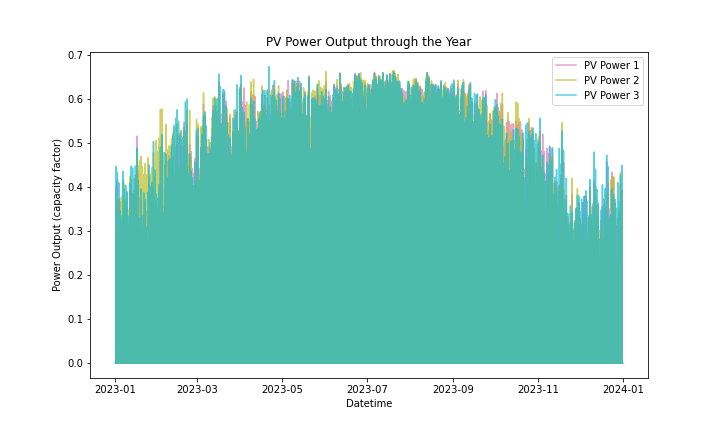
\includegraphics[width=\linewidth]{immagini/scenarios/PV_power_output_year.png}
  \caption{Solar Power Output (capacity factor)}
  \label{fig:PV year}
\end{subfigure}%
\quad
\begin{subfigure}{.45\textwidth}
  \centering
  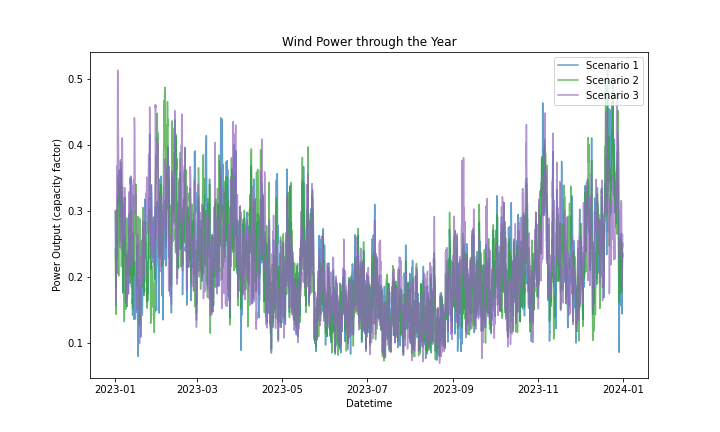
\includegraphics[width=\linewidth]{immagini/scenarios/wind_power_output_year.png}
  \caption{Wind Power Output (capacity factor)}
  \label{fig:wind year}
\end{subfigure}
\caption{Yearly Power Output of generated scenarios for Austria}
\label{fig: year power output}
\end{figure}

In Figure \ref{fig: few days power ouput} , we observe that both hour to hour and day-to-day interdependence is present in the generated scenarios, as there are instances of chained low solar production values. This accurately mimics the occurrence of cloudy days.

This characteristic is crucial for the yearly Wind Power distribution, as the Electrical Grid needs to have a higher storage capacity to compensate for the lower energy output. It must be noted that a less observed meteorological event in our scenarios, which is of great importance for renewable energy integration, is the Dunkelflaute, also known as Anticyclonic Gloom [\cite{Dunkelflaut}]. This event appears to be occurring more frequently due to climate change, implying a higher correlation between Wind and PV production, which could be modeled using the same Copula approach, although the growing size of the matrix \(\Sigma\) would need careful attention to keep the method computationally viable.

\begin{figure}[H]
\centering
\begin{subfigure}{.5\textwidth}
  \centering
  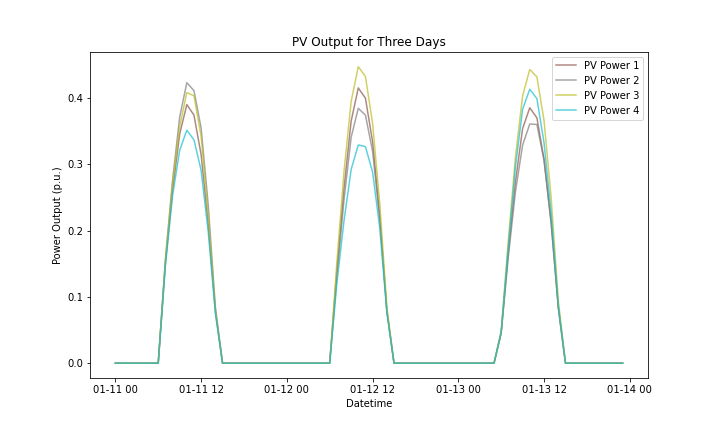
\includegraphics[width=\linewidth]{immagini/scenarios/PV_power_output_3days.png}
  \caption{Solar Power Output (capacity factor)}
  \label{fig:PV few days}
\end{subfigure}%
\begin{subfigure}{.5\textwidth}
  \centering
  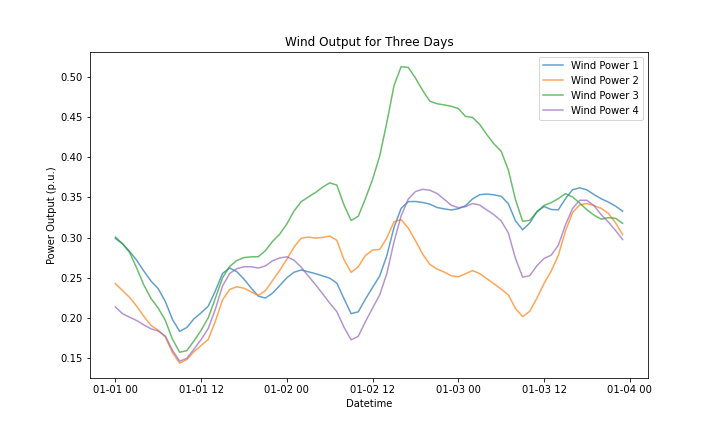
\includegraphics[width=\linewidth]{immagini/scenarios/wind_power_output_3days.png}
  \caption{Wind Power Output (capacity factor)}
  \label{fig:wind few days}
\end{subfigure}
\caption{3 days Power Output of generated scenarios for Austria}
\label{fig: few days power ouput}
\end{figure}






\section{Model Description}
\label{section: model}

The model describes a network in Europe that is to be powered and supplied of hydrogen trough power generated 
by photovoltaic panels and wind turbines, converted to hydrogen through electrolysis and potentially 
reconverted in fuel cells. It describes the handling of hydrogen throughout a one year time span, with
 one hour time steps, in order to meet demand.

The network is represented by an undirected multigraph \(\cG = (\cN, \cE)\), where \(\cN\) corresponds to the
 nodes in the network, and \(\cE = \cE_H \cup \cE_P\) represents transmission lines (\(e \in \cE_P\)) and
  hydrogen lines (\(e \in \cE_H\)). Each of these nodes can be in different countries in Europe, and the power
   generated by wind and solar power depends on the node location. In particular, if node \(n \in \cN\) is in
    France, the scenarios for power generation at \(n\) will be generated using parameters fitted to France's 
    data.

The operation of the Electric Grid is modeled as a two-stage stochastic program. In the first stage,
the capacity expansion of each generator, hydrogen storage, transmission line, and hydrogen pipe is
decided. In the second stage, the economic dispatch is solved for each scenario.






\newpage


%%%%%%%%%%%%%%%%%%%%%%%%%%%%%%%  VARIABLES  %%%%%%%%%%%%%%%%%%%%%%%%%%%%%%%%%%%%%

\subsection{Decision Variables}
The main variables that are of interest to the policy maker and are explicitly returned in output are the following:
\begin{align*}
    \text{ns}_n & : \text{Number of solar units (integer) at node } n \in \cN; \\
    \text{nw}_n & : \text{Number of wind units (integer) at node } n \in \cN; \\
    \text{nh}_n & : \text{Storage capacity (kg) (continuous) at node } n \in \cN;
\end{align*}
Stored hydrogen is considered to be the total of liquid and gas hydrogen to be stored. Our model does not assume a distinction between the two forms, and considers hydrogen to be immediately ready for long-term storage as soon as it is converted from electricity, as well as instantaneously convertible to electricity in fuel cells at need.

To give an indication of how much hydrogen should be kept in gas form at fuel cells, ready to be converted, and how much storage for gas hydrogen should be availlable at electrolyzers to accomodate abundant generation moments, we consider the following decision variables as well (N.B.: they are values \textit{per hour}, to be compared to the time necessary for gas to liquid hydrogen transformation and vice versa):
\begin{align*}
    \text{mhte}_n & : \parbox[t]{0.70\textwidth}{
    Maximum hydrogen to electricity capacity (Kg) (continuous), i.e. the maximum amount of hydrogen that needs to be converted within a 1h time frame into electricity at node} n \in \cN; \\
    \text{meth}_n & : \parbox[t]{0.70\textwidth}{Maximum electricity to hydrogen capacity (MWh) (continuous) at node} n \in \cN;
\end{align*}

To accommodate for possible improvements on capacity of existing power lines or hydrogen transport infrastructure, the following variables are added:
\begin{align*}
    \text{addNTC}_l & : \text{additional net transfer capacity on line $l$;}\\
    \text{addMH}_l & : \text{additional hydrogen transfer capacity on pipe $l$}.
\end{align*}
And parameters for the cost of such new infrastructure have to be given, indexed by edge of the respective graph: $cNTC_l$ and $cMH_l$.\\


The second stage variables, indexed by scenario \(j\), time step \(t\), and node \(n \in \cN\) are:
\begin{align*}
    \text{H}_{j,t,n} & : \text{Stored hydrogen at time \(t\), scenario \(j\) and node \(n\) (kg) (continuous)};\\
    \text{HtE}_{j,t,n} & : \text{Hydrogen converted to electricity at time \(t\),scenario \(j\) (kg) (continuous);} \\
    \text{EtH}_{j,t,n} & : \text{Electricity converted to hydrogen at time \(t\), scenario \(j\) (MWh) (continuous);}
\end{align*}
Note: all variables are set to be non-negative.


%%%%%%%%%%%%%%%%%%%%%%%%%%%%%%%  PARAMETERS  %%%%%%%%%%%%%%%%%%%%%%%%%%%%%%%%%%%%%

\subsection{Parameters} \label{subsection: Parameters}

There are a series of parameters that characterize the model and can be modified by the policy maker through the GUI. The main ones are related to capital costs of the infrastructure to be built:
\begin{align*}
    \text{cs}_n & : \text{Cost of one Solar Panel (\euro);} \\
    \text{cw}_n & : \text{Cost of one Wind Turbine (\euro)}; 
\end{align*} % Ciao Bia <3
If not specified through the GUI, the following values are assumed for panels and turbines: cs = 400\euro, cw = 3 000 000\euro. In this model we assume no marginal costs for PV and wind power production: the operating costs of the farms throughout their life-cycle can be factored into the capital costs, and there is no additional cost linked to the production itself. 
We assume the flow of electricity has no marginal cost nor power loss (the modelling of that problem is beyond the scope of this project). Conversely, we do set a cost for the use of hydrogen pipes (or other means of transfer):
\[
\text{cH\_edge}_l\ :\ \text{Cost of transferring 1kg of hydrogen through edge $l$}.
\]


Conversely, the marginal costs of conversion within electrolyzers and power cells are relevant. Thus one can set the following parameters:
\begin{align*}
    \text{chte} & : \text{Conversion cost of 1 kg of hydrogen to electricity (\euro/kg);} \\
    \text{ceth} & : \text{Conversion cost of 1 MWh of electricity to hydrogen (\euro/MWh).}
\end{align*}
According to the European Hydrogen Market Landcape November 2023 Report  \cite{European_H2_Market_landscape},
 ``Hydrogen production costs via electrolysis with a direct connection to a 
 renewable energy source in Europe vary from 4.18 to 9.60 €/kg H2 of hydrogen, with the average
  for all countries being 6.86 €/kg H2''. For electrolyzers, we consider the Levelised cost of hydrogen (LCOH)
   to account for both marginal costs and capital costs. Such cost is dependent on the country's specific market
    condition and can be calculated through the \href{https://observatory.clean-hydrogen.europa.eu/tools-reports/levelised-cost-hydrogen-calculator}{European Hydrogen Observator tool}. Unless specified through the GUI, $ceth$ = 20kg/MWh*10\euro/kg=200\euro/MWh is assumed (see the discussion on conversion efficiency below), and $chte$ is assumed to be 2\euro/kg. 
Furthermore, the storage of the hydrogen itself has a cost that depends on various factors: capital cost of the technology used for storage, operating costs, length of time that the hydrogen is kept in storage. Thus the following parameters can be set:
\begin{align*}
    \text{ch} & : \text{Cost of hydrogen storage capacity per unit of hydrogen (\euro/kg);} \\
    \text{ch\_t} & : \text{Cost of storing hydrogen for 1h, per unit of hydrogen (\euro/(kg$\cdot$h)).}
\end{align*}
Thus $ch$ will be simply multiplied by the maximum storage needed ($nh$), representing capital
 cost of storage infrastructure, whereas $ch\_t$ represents the marginal cost of keeping the
  hydrogen stored.  Unless specified, it is assumed to be $ch=10$\euro/kg and $ch_t=0$\euro/(kg$\cdot$h)

Within the electrolyzers and fuel cells, the conversion itself can be more or less efficient:
\begin{align*}
    \text{fhte} & : \text{efficiency of hydrogen to electricity conversion (scalar between 0 and 1);} \\ 
    \text{feth} & : \text{efficiency of electricity to hydrogen conversion (scalar between 0 and 1).}
\end{align*}
It is assumed that 1kg of hydrogen has an energy value of 33kWh. Thus if we consider an electrolyzer operating at maximum efficiency ($feth=1$), one MWh of electricity yields 1000/33$\simeq$30kg of hydrogen. If not specified through the GUI, a value of $feth=0.66$ is considered, thus 1MWh yields 20kg of hydrogen.
Conversely, in a fuel cell operating at maximum efficiency ($fhte=1$) 1kg of hydrogen yields 
33kWh. If not specified through the GUI, a value of $fhte=0.75$ is considered, yielding 24.75kWh 
per kg of hydrogen. Actual efficiencies vary a lot depending on the technology used. Furthermore, chemical
 and physical constraints make it so that efficiencies higher than 0.80-0.85 are currently considered 
 unachievable \cite{DAWOOD}.

Finally, the GUI gives the option to place upper bounds to the variables, based on either technological and physical constraints (dimension of the facilities) or because of political choices (local population unfavourable to wind turbines): 
\begin{align*}
    \text{Mns} & : \text{Maximum number of solar panels that can be installed (integer);} \\ 
    \text{Mnw} & : \text{Maximum number of wind turbines that can be installed (integer);} \\ 
    \text{Mnh} & : \text{Maximum hydrogen storage capacity (kg);}\\
    \text{Mhte} & : \text{Upper bound for \(mhte\) (kg)}; \\ 
    \text{Meth} & : \text{Upper bound for \(meth\) (MWh)}.
\end{align*}
If no bound is given through the GUI, these values will be set to $Mns=10^6, Mnw=500, Mnh=10^9, Mhte=10^6, Meth=10^5)$. Note: computation time increases significanly when increasing the upper bound for $Mnw$.

A scenario consists in a different realizations of the following variables, given as input in the model and  indexed by scenario \(j\), time step \(t\), and node \(n \in \cN\):
\begin{align*}
    \text{ES}_{j,t,n} & : \text{Power output of a single solar panel (MWh)}\\
    \text{EW}_{j,t,n} & : \text{Power output of a single wind turbine (MWh)}\\
    \text{EL}_{j,t,n} & : \text{Electricity load (MWh)}\\
    \text{HL}_{j,t,n} & : \text{Hydrogen load (kg)} \\
    \text{P\_edge}_{j,t,l} & : \text{Power passing through line $l$ during time step $t$ in scenario $j$ (MWh) (continuous)};\\
    \text{H\_edge}_{j,t,l} & : \text{Hydrogen flowing through pipe $l$ during time step $t$ in scenario $j$ (kg) (continuous)}.
\end{align*}

Lastly the following parameters are indexed by edge of the respective graph:
\begin{align*}
    \text{NTC}_l : & \ \parbox[t]{0.65\textwidth}{Net Transfer Capacity, that is, maximum amount of electricity that can pass on line \text{$l$} of the electric grid in the span of 1h;}\\
    \text{MH}_l : & \text{ Maximum amount of hydrogen that can flow on edge $l$ in 1h}.
\end{align*}
\subsubsection{Objective Function}
The cost function is given by the sum of all capital costs of installing infrastructure, all marginal costs of the hour-by-hour hydrogen to electricity and electricity to hydrogen conversions, and minimal costs associated to the variables $mhte$ and $meth$ so that they are minimized through the model.
% \begin{align*}
%     \min \quad & \text{cs} \cdot \text{ns} + \text{cw} \cdot \text{nw} + \text{ch} \cdot \text{nh} + \\
%     & + \frac{1}{d}\sum_{j=1}^{d} \sum_{i=1}^{\text{inst}} (\text{ch\_t} \cdot \text{H}_{j,t} + \text{chte} \cdot \text{HtE}_{j,t} + \text{ceth} \cdot \text{EtH}_{j,t}) +\\
%     & + 0.01*(mhte + meth).
% \end{align*}
Let $Nnodes$, $NEedges$ and $NHedges$ be the number of nodes, edges on the electric grid graph and edges of the hydrogen transfer graph respectively. The objective function is modified as follows:
\begin{align*}
    \min \quad 
    &&\sum_{k=1}^{\text{Nnodes}}&\text{cs}_k \cdot \text{ns}\hspace{-3.5em}&&_k+\text{cw}_k \cdot \text{nw}_k + \text{ch}_k \cdot \text{nh}_k + \\
    &+& \sum_{l=1}^{\text{NEedges}}& \text{cNTC}_l \hspace{-3em}&&\cdot\text{addNTC}_l 
    + \sum_{l=1}^{\text{NHedges}} \text{cMH}_l\cdot \text{addMH}_l + \\   
    &+&\frac{1}{d}\sum_{j=1}^{d}&\sum_{i=1}^{\text{inst}} \Bigg( \hspace{-5em}&&
    \sum_{k=1}^{\text{Nnodes}} (\text{ch\_t}_k \cdot \text{H}_{j,t,k} + \text{chte}_k \cdot \text{HtE}_{j,t,k} + \text{ceth}_k \cdot \text{EtH}_{j,t,k}) + \\
    &&&\hspace{-2em}&&+\sum_{l=1}^{\text{NHedhes}} (\text{cH\_edge}_l\cdot\text{H\_edge}_{j,t,l}) \Bigg) + \\
    &+&\sum_{k=1}^{\text{Nnodes}}& 0.01\cdot(\hspace{-2.8em}&&mhte_k+meth_k)
\end{align*}

The $1/d$ factor in front of the marginal costs allows to average over the scenarios, whereas the capital costs are the same for all scenarios. Thus, ignoring the costs of $mhte$ and $meth$, the objective function value gives an estimate of the actual costs (in \euro) for the set up and maintenance of the system throughout the length of the scenario (one year). 
%%%%%%%%%%%%%%%%%%%%%%%%%%%%%%%  CONSTRAINTS  %%%%%%%%%%%%%%%%%%%%%%%%%%%%%%%%%%%%%

\subsection{Constraints}
The following constraints are to ensure that for all time steps $t$ and all scenarios $j$, the electricity load and the hydrogen load are met. The measure units are MWh and kg respectively, conversion factors are considered for $HtE$ and $EtH$ respecively.
Let $Out(n)$ and $In(n)$ indicate the outgoing and incoming edges from node $n$ on the respective graph. Then for each node $n$, the we have the following flow balance constraints:
\begin{align*}
    \text{Electricity Balance:} \quad & \text{ns}_n \cdot \text{ES}\hspace{-1em}&_{j,t,n}&+ \text{nw}_k \cdot \text{EW}_{j,t,n} + 0.033 \cdot fhte_k \cdot \text{HtE}_{j,t,n} - \text{EL}_{j,t,n} - \text{EtH}_{j,t,n} + \\
    & \sum_{l\in Out(n)}\hspace{-1em}& \text{P\_e}&\text{dge}_{j,t,l} + \sum_{l\in In(n)} \text{P\_edge}_{j,t,l} \ge 0;\\
    \text{Hydrogen Storage:} \quad & \text{H}_{j,t+1,n} \hspace{-1em}&=\ & \text{ H}_{j,t,n} + 30 \cdot feth_k \cdot \text{EtH}_{j,t,n} - \text{HtE}_{j,t,n} - \text{HL}_{j,t,n} -\\ &&& - \sum_{l\in Out(n)}\text{H\_edge}_{j,t,l} + \sum_{l\in In(n)}\text{H\_edge}_{j,t,l}
\end{align*}

We ask that the consumed electricity be less or equal than the produced electricity at all times. On the grid itself, the two sides should be equal, but we observe that $ns\cdot ES_{j,t} + nw\cdot EW_{j,t}$ indicate the maximum power that can be generated with set weather conditions, whereas actual production will be regulated to meet demand through curtailment.

The stored hydrogen at time $t+1$ is the result of what was stored at time $t$ adjusted by what was converted and what was sent to the industrial load. For $t=24*365$ we set the same constraint on hydrogen by considering $t+1$ to be index $1$: this way we avoid placing a ``start time'' at an arbitrary place within the year (time is rendered modulo the year) and we avoid the model asking for conveniently high initial storage values of hydrogen appearing out of thin air.

The total storage and conversion capacities are calculated by minimizing the maximum over time and scenarios of the variables $H_{j,t}, EtH_{j,t}$ and $HtE_{j,t}$, for all scenarios \(j\), time steps \(t\) and nodes \(n\):

\begin{align*}
    \text{Storage Capacity Limit:} \quad & \text{H}_{j,t,n} \leq \text{nh}_n ;\\
    \text{EtH Conversion Limit:} \quad & \text{EtH}_{j,t,n} \leq \text{meth}_n;\\
    \text{HtE Conversion Limit:} \quad & \text{HtE}_{j,t,n} \leq \text{mhte}_n .
\end{align*}
Finally, edge capacities on the respective graphs are considered for all scenarios \(j\), time steps \(t\) and nodes \(n\):
\begin{align*}
    \text{Net Transfer Capacity:} \quad & |\text{P\_edge}_{j,t,l}|\le\text{NTC}_l + \text{addNTC}_l ;\\
    \text{Hydrogen Transfer Capacity:} \quad & |\text{H\_edge}_{j,t,l}|\le\text{MH}_l + \text{addMH}_l.
\end{align*}

\section{Optimization and Time Resolution}\label{section:time-resolution}

The time horizon generated by the scenarios has a time resolution where each time step has a length of one hour. Each value represents the total power (hydrogen) production or demand in the corresponding hour at the node. The smaller the length of each time step, the more accurate the results. However, the number of variables and constraints grows linearly with the number of time steps, making the model intractable (especially in the context of an application) with just a few scenarios.

Moreover, considering every hour in each day of the year is partly redundant, as each day will be similar to neighboring days. Yet, simply considering a sample of days for each season might undermine long-term storage capacity representation. 

Given an initial time horizon \(\cT = \{1, \ldots, T\}\), we can consider partitions of \(\cT\) as a family of disjoint subsets whose union is \(\cT\). We only consider those partitions where every subset is an interval of \(\cT\). We refer to these as time partitions. Given a time partition \(P\), we can consider the corresponding model obtained by considering each interval in \(P\) as a single time step. For every \(I\) in \(P\), we define:
\[
ES_{j,I,n} \coloneqq \sum_{i \in I} ES_{j,i,n}, \quad EW_{j,I,n} \coloneqq \sum_{i \in I} EW_{j,i,n}
\]
and similarly for \(HL_{j,I,n}\) and \(HR_{j,I,n}\). We denote the model obtained by the time partition \(P\) as \(CEP_P\).

It is evident that the optimal value of \(CEP_P\) is a lower bound for the original problem \(CEP_{\cT}\), as given a feasible solution \((ns, nw, nh, mhte, meth, H, HtE, EtH, Pedge, Hedge)\) of the latter, we can obtain a solution of the former by taking \((ns, nw, nh, mhte, meth)\) the same as in \(CEP_{\cT}\) and:
\[
Pedge_{j,I,e} = \sum_{i \in I} Pedge_{j,i,e}, \quad Hedge_{j,I,e} = \sum_{i \in I} Hedge_{j,i,e}
\]
and similarly for \(EtH\) and \(HtE\), and \(H_{j,I,n} = H_{j,i_0,n}\) where \(I = [i_0,\ldots,i_{|I|}] \in P\). In particular, there is a cost-preserving linear map from the feasible space of \(CEP_{\cT}\) to the feasible space of \(CEP_P\), making the latter a relaxation of the former.

This is generally true when considering any time partition \(P'\) finer than \(P\), where for every \(t' \in P'\), there exists \(t \in T\) such that \(t' \subset t\). In particular, we have the following observation:

\begin{observation}
Let \(V_{\cP} \subset \bR^{N_{\cP}}\) and \(V_{P'} \subset \bR^{N_{P'}}\) be the space of feasible solutions of \(CEP_{\cP}\) and \(CEP_{P'}\), respectively. There exists a linear map \(L_{P'P}: \bR^{N_{P'}} \to \bR^{N_{P}}\) such that \(L(V_{P'}) \subset V_{P}\) and \(c_{P}(L(x)) = c_{P'}(x)\), where \(c_{P}\) is the cost function of \(CEP_{P}\) and \(c_{P'}\) is the cost function of \(CEP_{P'}\).
\end{observation}

Thus, by iteratively solving finer time partitions, we converge to the optimal solution of \(\cP\).

\subsection{Warmstart}
Let \(P'\) be a finer time partition than \(P\). Given an optimal basic feasible solution of \(CEP_{P}\), we can use it to efficiently warm start the solution of \(CEP_{\cP'}\). This is done by, keeping the variables and constraints of \(CEP_{P}\) and adding additional constraints to \(CEP_{\cP'}\) to further link the additional variables with those of \(CEP_{P}\). For every \(I \in P\), scenario \(j\), and edge \(k\), we add the following constraints to \(CEP_{P'}\):

\begin{align*}
  \text{EtH}_{j,I,k} &= \sum_{J \in P'(I)} \text{EtH}_{j,J,k} \\
  \text{HtE}_{j,I,k} &= \sum_{J \in P'(I)} \text{HtE}_{j,J,k} \\
  \text{P\_edge}_{j,I,k} &= \sum_{J \in P'(I)} \text{P\_edge}_{j,J,k} \\
  \text{H\_edge}_{j,f,k} &= \sum_{J \in P'(I)} \text{H\_edge}_{j,J,k}
\end{align*}

We observe that these constraints imply \(H_{j,I,k} = H_{j,J_0,k}\) where \(J_0\) is the leftmost interval of \(I\). This is coherent with the interpretation that \(H_{j,I,k}\) corresponds to the initial hydrogen storage in the interval \(I\). This can be seen by summing over \(J\) the hydrogen storage constraint %(\textcolor{red}{ref}):
\begin{align*}
 0 & = \sum_{i=0}^{|P'(I)|-1}\bigl(\text{H}_{j,J_{i+1},n}  - \text{ H}_{j,J_{i},n} + 30 \cdot feth_k \cdot \text{EtH}_{j,J_{i},n} - \text{HtE}_{j,J_{i},n} - \text{HL}_{j,J_{i},n} \\
&- \sum_{l \in \text{Out}(n)} \text{H\_edge}_{j,J_{i},l}  + \sum_{l \in \text{In}(n)} \text{H\_edge}_{j,J_{i},l} \bigr) =  \\  
&=   \text{H}_{j,J_{i+1},n}  - \text{ H}_{j,J_{0},n} + 30 \cdot feth_k \cdot \text{EtH}_{j,I,n} - \text{HtE}_{j,I,n} - \text{HL}_{j,I,n}  \\ 
&-\sum_{l \in \text{Out}(n)} \text{H\_edge}_{j,I,l}  + \sum_{l \in \text{In}(n)} \text{H\_edge}_{j,I,l} \\ 
&= \text{H}_{j,J_{i+1},n}  - \text{ H}_{j,I, n} + 30 \cdot feth_k \cdot \text{EtH}_{j,I,n} - \text{HtE}_{j,I,n} - \text{HL}_{j,I,n} \\
&- \sum_{l \in \text{Out}(n)} \text{H\_edge}_{j,I,l}  + \sum_{l \in \text{In}(n)} \text{H\_edge}_{j,I,l}
\end{align*}

Due to the linearity of the objective function, we do not need to modify the cost vector of \(CEP_P\). Given an optimal basic feasible solution of \(CEP_P\) with basis \(B\), we can obtain a basic solution of \(CEP_{P'}\) by simply adding the columns corresponding to the variables EtH and HtE. This results in a basic solution of \(CEP_{P'}\) with basis \(B'\).

Although this solution is not necessarily feasible for \(CEP_{P'}\), the block structure of \(B'\) and the unchanged cost vector ensure that the reduced cost vector remains negative. Consequently, we can obtain a dual feasible solution given by \(c_{B'} B'^{-1} b\), where \(b\) is the constant vector of \(CEP-P'\), which can be used as a warm start for the dual simplex algorithm.

%%%%%%%%%%%%%%%%%%%%%%%RESULTS%%%%%%%%%%%%%%%%%%%%%%%%%%%%%%%%%%%%%%%%%%%%%%
\section{Results}


In this section, we present a series of numerical experiments, which can be reproduced by configuring the network to "small-eu" in the application \cite{MOPTA}. The model is solved using Gurobi, with computation times measured on a computer equipped with a 13th Gen Intel(R) Core(TM) i7-13700H processor running at 2.40 GHz and 16 GB of installed RAM.
\begin{figure}[H]
\begin{subfigure}{0.5\textwidth}

\vspace{-10pt}

  The example model is a five node network consisting of 5 nodes in different countries: France, Germany, Spain, Italy, and Austria and subject to different wheather and load conditions.

\end{subfigure}
\begin{subfigure}{0.5\textwidth}
\centering
\vspace{-10pt}
\includegraphics*[width=0.5\textwidth]{immagini/small-eu-network.png}
\end{subfigure}
\caption{Small-eu network}
\label{fig:small eu network}
\end{figure}
\subsection{Time partition results}
While the algorithm described in Section \ref{section:time-resolution} details how successive iterations can be efficiently warm-started, this section provides guidance on selecting the initial time partition and the iteration method. Specifically, the iteration method refers to the strategy used to decide which time intervals in the current partition should be split into smaller intervals.

Regarding the initial time partition, we compare two different strategies against the finest partition \(\cT\), where each time step is one hour long. This finest partition offers the highest accuracy but is also the most computationally demanding.

The first partition, \(\cT_1\), groups all days together except for ten evenly spaced days, where each hour is treated as a separate interval. The second partition, \(\cT_2\), divides each day into two intervals: one for daylight hours and one for night hours. This approach is motivated by the fact that solar power generation occurs only during daylight hours.

In both cases, \(\cT_1\) and \(\cT_2\), the finest partition \(\cT\) is used as the reference for comparison.
We observe that there is no particular difference between the two partitions, in fact, surprisingly they yeald the same results and are solved in a similar time (22s), while the model with \(\cT\) time partition takes a longer time to solve (320s).
The main difference between \(\cT_1\) and \(\cT_2\) is that the latter seems to better rapresent the daily and seasonal variations of hydrogen storage as can be seen in Figure \ref{fig:aggHydrogen}. The difference between the cost of the relaxed models of \(\cT_1\),\(\cT_2\) and of \(\cT\) is of order 10\%.
Thus, to obtain a better approximation of the optimal solution, we iteratively refine the time partitions.

\begin{figure}[H]
  \centering
  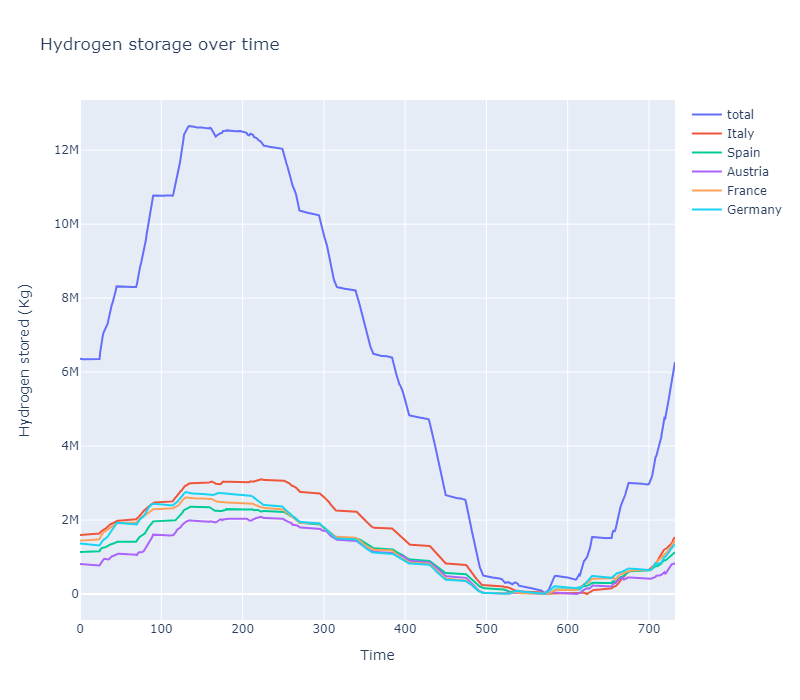
\includegraphics[width=0.30\textwidth]{immagini/time_aggregation/agg2hydrogen.png}
  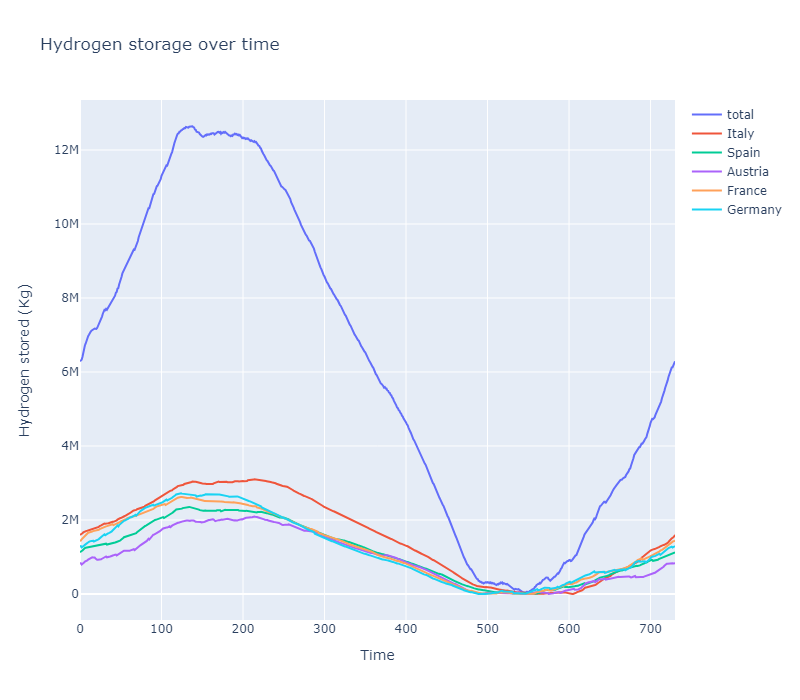
\includegraphics[width=0.30\textwidth]{immagini/time_aggregation/agg1hydrogen.png}
  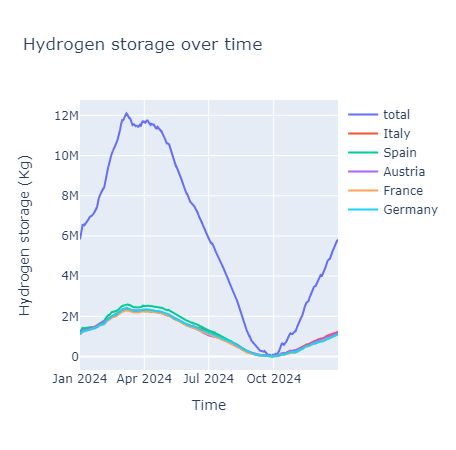
\includegraphics[width=0.30\textwidth]{immagini/time_aggregation/finesthydrongen.png}
  \caption{Comparison of hydrogen storage aggregation \(\cT_1,\cT_2\) and \(\cT\).}
  \label{fig:aggHydrogen}
\end{figure}

The iteration method we tested involves randomly selecting a time interval and splitting it into one-hour
intervals. While this approach appears to be slightly faster on average than directly optimizing on the final
time partition, it can produce suboptimal results when compared to time partitions of similar lengths.
To reliably use this method, a validation function needs to be developed to identify which time interval has most violated constraints.
\subsection{Analysis of the results}

Within a day, we can observe that the stored hydrogen is used to satisfy demand up until dawn: at this point, PV power starts to supply our load and along with generated wind power is enough to refill the depleted hydrogen storage and add to it. In the evening, when the sun sets and electricity load is still high, some of the stored hydrogen is again used to fulfill hydrogen and energy demand. We observe the noticable weekly trend in electricity load, with lower demand on weekends. 


When looking at the full year, we can see the seasonal trends in both weather (and thus generation) and demand are depicted in Figure \ref{fig:energytrends}. The winter has much higher demand with lower PV power generation, but higher wind power generation. Still, the solution by the solver indicates that it is convenient to store hydrogen during the summer and to use it during winter.\\


\begin{figure}[H]
  \centering
  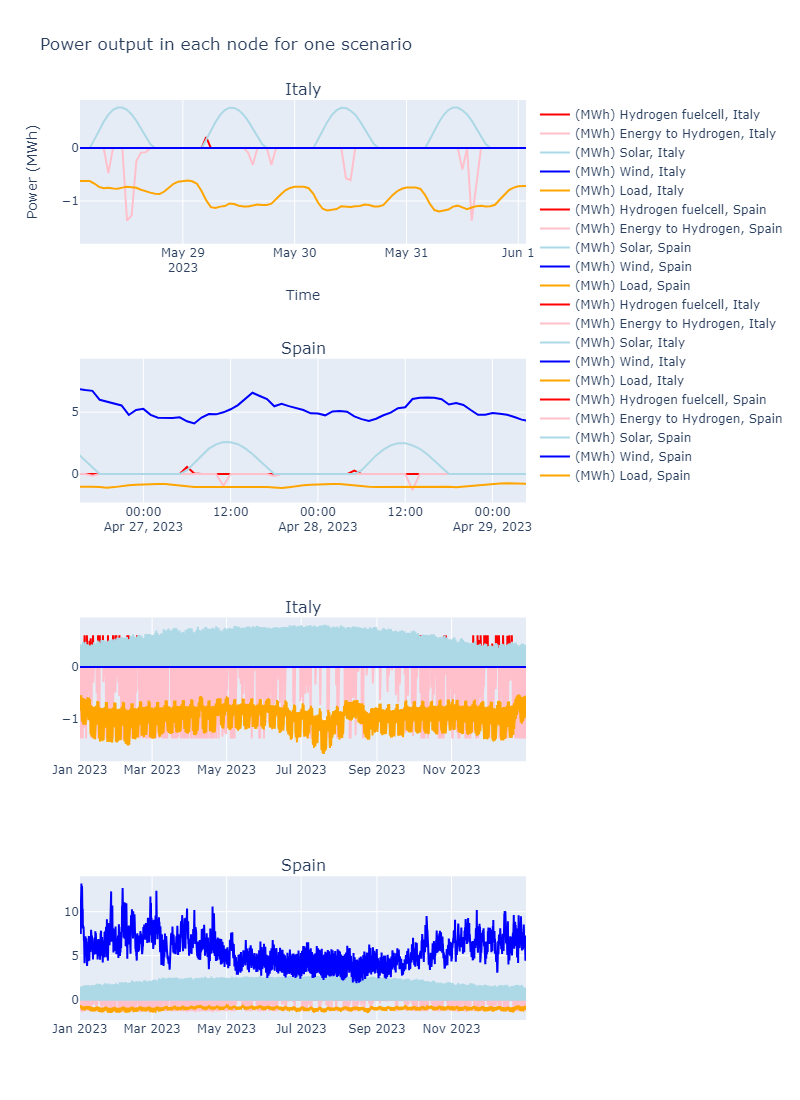
\includegraphics[width=0.80\textwidth]{immagini/ImmaginiOptimization/image1.png}
  \caption{Energy trends in the network, The y-axis represents energy generation and load in MWh.}
  \label{fig:higheffenergytrends}
\end{figure}
We observe that Hydrogen efficiency plays a big role in the structure on the network. Low hydrogen efficienty networks tend to have a higher diversity in energy sources to compansate for their variability (as can be seen in \ref{fig:energytrends}), since a lot of energy is lost when converting from energy to hydrogen and then back to energy. We observe that the various nodes tend to have one main type of energy source, depending on the country they are located in. This suggests that high collaboration between countries is required to achieve the best results, but this is only a feasible solution when high amounts of transmission between countries is possible (high NTC values).

\begin{figure}[H]
  \centering
  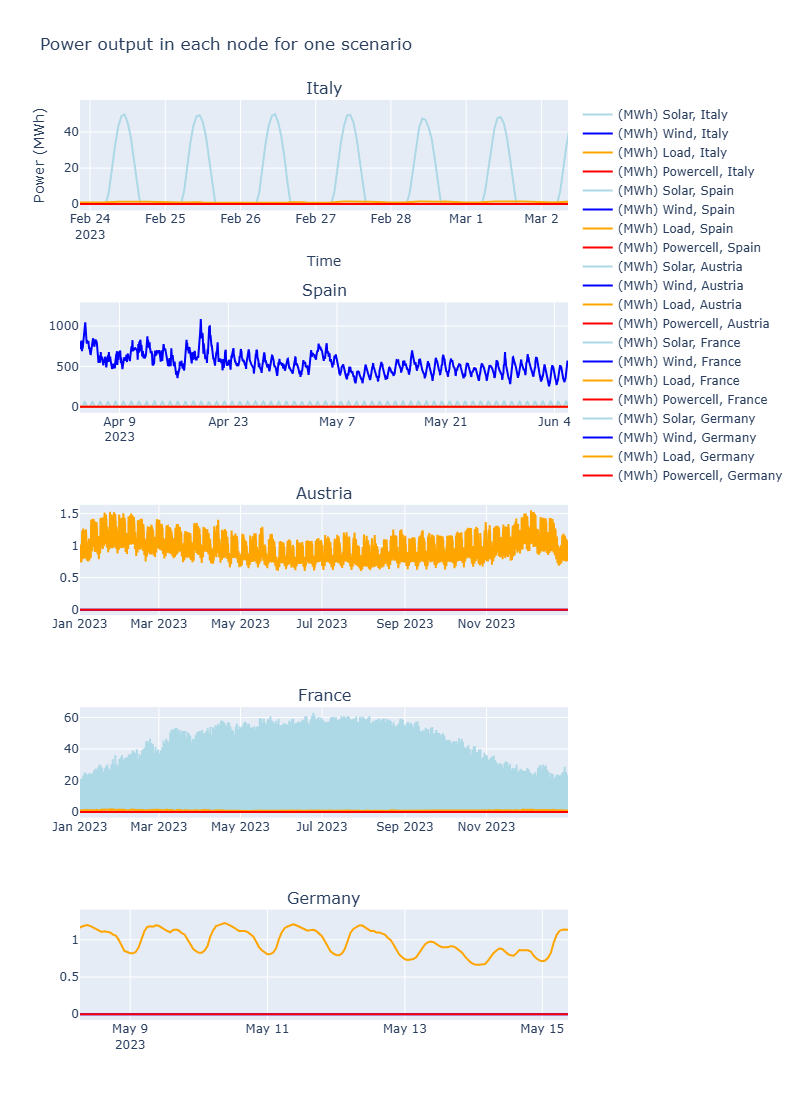
\includegraphics[width=0.80\textwidth]{immagini/time_aggregation/Energytrends.png}
  \caption{Energy trends in the network, The y-axis represents energy generation and load in MWh.}
  \label{fig:energytrends}
\end{figure}



\subsection{Future directions and conclusion.}

To enhance the realism and applicability of our energy models, future improvements will focus on integrating wind and solar power scenarios with energy demand models. The parametric modeling of the marginal distributions of solar and wind power provides a robust foundation for incorporating the impacts of climate change. By analyzing shifts in distribution parameters over time, we can adapt our models to better forecast changes in energy production capabilities. Additionally, we plan to extend this approach to account for spatial and generator-type interdependencies. Leveraging real-time data directly from the grid will offer a more nuanced understanding of how various renewable energy sources interact across different timescales and spatial dimensions.

As the number of interdependent variables modeled with the copula approach increases, there is a risk of encountering poor results due to the curse of dimensionality. To address this, one research direction is to approximate the covariance matrix as a banded matrix, thereby reducing the problem's dimensionality. This approach is supported by the assumption that time steps far apart are not significantly correlated. Projection methods can be employed to ensure the matrix remains positive semidefinite. A basic implementation of this was used to save efficiently the covariance matrices.

Another direction for improvement consists in manually constructing the initial solution to warm start the model at each iteration, as Gurobi's warm-start efficiency decreases as the number of scenarios grows. Moreover, while we currently use the same time partition for all scenarios, a more effective approach would involve treating each scenario’s time partition independently by identifying the specific time intervals where constraints are violated.

To create a more realistic model, this method could be readily extended to a DC Optimal Power Flow (OPF) framework, though doing so would significantly increase the complexity of the problem. Additionally, from the perspective of policymakers, it would be valuable to incorporate various types of green energy sources into the network. For example, adding hydropower could provide additional energy storage, while geothermal and nuclear energy with their consistent energy supply could reduce the dependence on storage solutions and reduce material consumption.
%\subsection{Results and validation}
% \subsection{Results for single node network}

% We first test our model on the example of a random weather scenario in Belgium, with electricity demand from 2023. We solve for a whole year, and then look at what happens on a single day, over the course of a month, and throughout the whole year. We plot the results in figure \ref{fig: plot Belgium}. On the top right we plot the power generated through PV panels and wind turbines as the product between the hourly power per unit we gave as input and the number of panels and turbines we got as output respectively. The top left plots display electric and hydrogen loads, given to the model as input. On the bottom we plot the time series of the hydrogen contained in storage.


% \begin{figure}[H]
% \centering
% \begin{subfigure}{.30\textwidth}
%   \centering
%   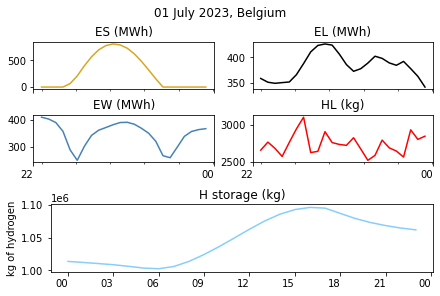
\includegraphics[width=\linewidth]{immagini/Single_node/Belgium_01_07.png}
% \end{subfigure}%
% \quad
% \begin{subfigure}{.30\textwidth}
%   \centering
%   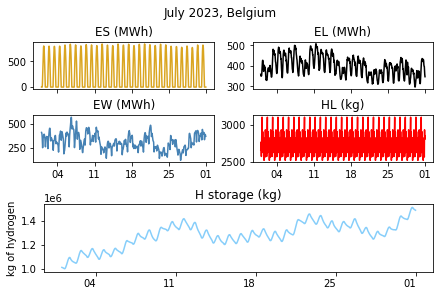
\includegraphics[width=\linewidth]{immagini/Single_node/Belgium_07.png}
% \end{subfigure}
% \quad
% \begin{subfigure}{.30\textwidth}
%   \centering
%   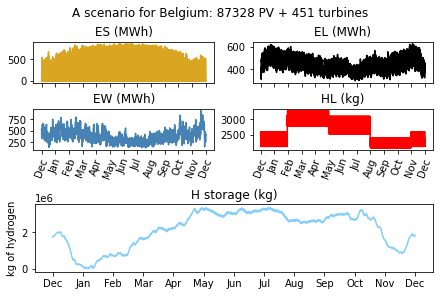
\includegraphics[width=\linewidth]{immagini/Single_node/plot_BE_all.png}
% \end{subfigure}%
% \caption{Inputs and resulting hydrogen storage for a day, a month and a year in Belgium}
% \label{fig: plot Belgium}
% \end{figure}



% On a single scenario, we find trends we were expecting. We are now interested in evaluating the stability of the solution regarding the decision variables linked to infrastructure. We  In figure \ref{fig: sols_BE} we plot the number of turbines against the number of PV panels for the cases considered, and beneath we look at the normalized distribution of the output values for $meth$, $mhte$, and $nh$.

% \begin{figure}[H]
% \centering
% 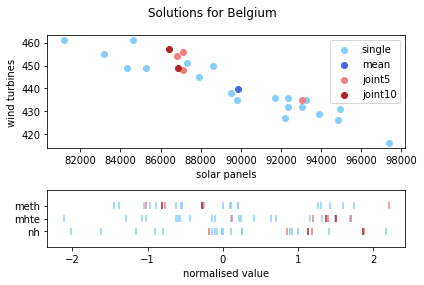
\includegraphics[width=0.75\textwidth]{immagini/Single_node/sols_BE.png}
% \caption{Outputs for various scenarios, Belgium}
% \label{fig: sols_BE}
% \end{figure}




% \subsection{Results for integrated network}
% \subsubsection{Relevance of integration}
% Comparison of total cost for the network vs sum of costs with opt1 for each state, that is. Hopefully we show "collaboration good".

% \subsubsection{Case study: EU}
% Test on EU network: get the max capacities from 

% Tesi magistrale del tipo che ha fatto mini analisi su quanto sono effettivamente utili i progetti di integrazione della rete elettrica europea: cito perché sto seguendo il suo esempio nel recuperare i dati sulle capacità delle linee
% \hyperlink{https://www.diva-portal.org/smash/get/diva2:1476768/FULLTEXT01.pdf}{\textcolor{blue}{link}} (pagina 30). Pagina da cui scaricare i dati a cui si riferiva:
% \hyperlink{https://transparency.entsoe.eu/transmission-domain/physicalFlow/show?name=&defaultValue=false&viewType=TABLE&areaType=BORDER_CTY&atch=false&dateTime.dateTime=22.07.2024+00:00|CET|DAY&border.values=CTY|10YGR-HTSO-----Y!CTY_CTY|10YGR-HTSO-----Y_CTY_CTY|10YIT-GRTN-----B&dateTime.timezone=CET_CEST&dateTime.timezone_input=CET+(UTC+1)+/+CEST+(UTC+2)}{link}.

% Then save decision variables addNTH$_l$ to check where investment is most needed. La tesi magistrale del tipo poi ha una lista di progetti in corso, per vedere se l'UE si sta comportando in modo sensato.

% % \subsubsection{Attempts at a validation function}
% As for the single node case, while computing the optimal solution on a batch of scenarios, the solver ``knows the future'' for those scenarios. That is, the criteria it uses to determine, at each time step, how much electricity or hydrogen should be converted or transmitted, and where, is a mathematical minimum that is informed by the knowledge of what is needed at any time during the one year scenario. In the single node scenario, this did not pose much of a problem when designing a validation function to test the infrastructure on new scenarios. That is because the actions and choices of a power grid administrator of an isolated grid are very much limited to ``if I have extra energy, I store it, up to storage limit''. This is not true anymore once you take the node out of isolation: at each moment, without knowledge of the full future, each fictional administrator at each node must choose whether to store the energy generated at their node, whether to send it to a neighbour (and how much to which neighbour) or how to collect missing energy to match their node's demand.\\


% Our first attempt at a validation function was to simply fix the values of the decision variables linked to infrastructure, and resolve the problem on a new scenario with the solver for all time dependent decision variables. This solution does obviously evaluate feasibility in a mathematically precise way (it determines whether there exists a solution), but it doesn't solve our problem: it doesn't offer much insight into how humans could actually replicate that solution in real life, without knowledge of the future.\\

% <<< results with such validation function?? >>>> \textcolor{red}{TO DO}\\

% A more realistic attempt, though computationally monstrous, could be the following:
% Assume we have a two day forecast, optimize on that every two days, do what the solution says for two days, then set your new state as initial conditions for a new 2day-optimization problem.\\

% This is a procedure that could actually be followed by humans. The cost evaluated through this could be a realistic estimate of the actual cost

% Even better:
% Solve the problem for the average scenario. Save the time dependent results. When optimizing over the two day period, add a loss function using the distance from the average scenario.



% \newpage
% \section{Cose scritte prima che sto spingendo in fondo}
% \subsection{Dependence on the parameters?}
% The result of the Energy Grid simulation greatly varies depending on the values of the parameters described in \ref{subsection: Parameters}. In this section we try to explicate this dependence.

% %\subsection{Diverse Energy Grid}
% A Diverse Energy Grid, that is a grid in which more than one type of generator is present is obtained with the following parameters:

% \begin{center}
% \begin{tabular}{ c c c c c c c c c c c c }

%  cs (€)& cw (€)& Mns& Mnw& Mnh (kg)& ch (€)& chte (€)& fhte& Mhte& ceth (€)& feth& Meth \\ 
%  4000 & 3000000 & \(\infty\) & \(\infty\) & \(\infty\) & 10 & 2 & 0.75 & \(\infty\) & 200 & 0.7 & \(\infty\) \\  
% \end{tabular}
% \end{center}

% In Figure \ref{fig:balanced year}, we observe that hydrogen storage is accumulated during periods when the main power source, wind power in this case, generates excess energy. Conversely, the stored hydrogen is depleted during periods of low power output. It's important to note that this process doesn't rely on the operator's foresight of future events. At each time step, no decision is made on whether to store hydrogen or not. Instead, any excess energy is automatically converted into hydrogen, or it is lost if the conversion capacity is insufficient. \textcolor{red}{questo nella funzione di validazione hehe}

% \begin{figure}[H]
% \centering
% \begin{subfigure}{.5\textwidth}
%   \centering
%   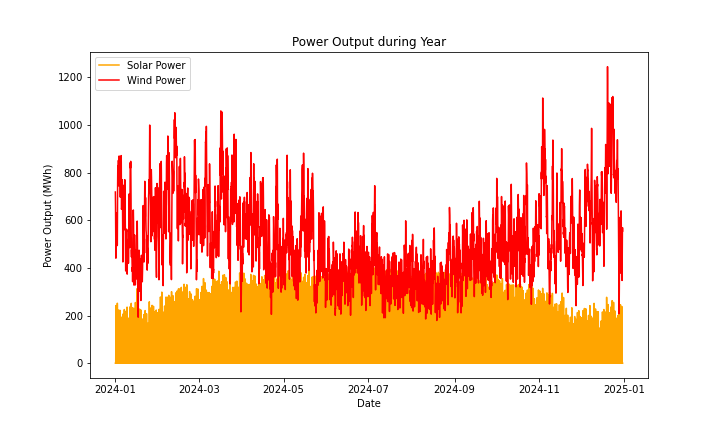
\includegraphics[width=\linewidth]{immagini/ImmaginiOptimization/balancedPowerOutput.png}
%   \caption{Solar and Wind Power Output (MWh)}
%   \label{fig:balance year power}
% \end{subfigure}%
% \begin{subfigure}{.5\textwidth}
%   \centering
%   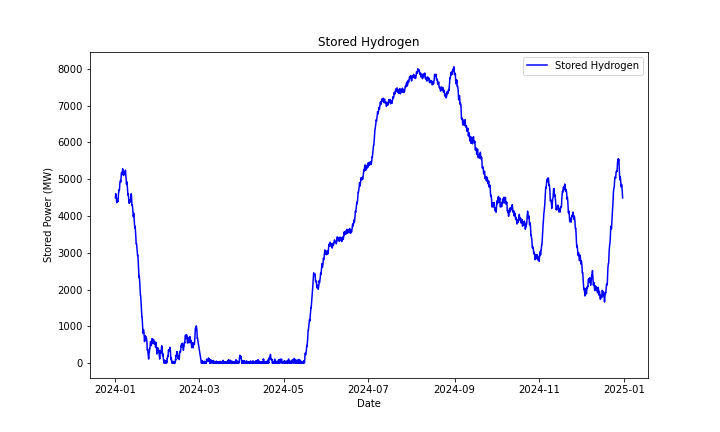
\includegraphics[width=\linewidth]{immagini/ImmaginiOptimization/HHyear.png}
%   \caption{Hydrogen Storage (MW)}
%   \label{fig:balanced year hydrogen}
% \end{subfigure}
% \caption{Annual Power Production and Storage)}
% \label{fig:balanced year}
% \end{figure}

% In Figure \ref{fig:balanced day}, we observe daily fluctuations in hydrogen storage due to the decrease in solar power production at night.


% \begin{figure}[H]
% \centering
% \begin{subfigure}{.5\textwidth}
%   \centering
%   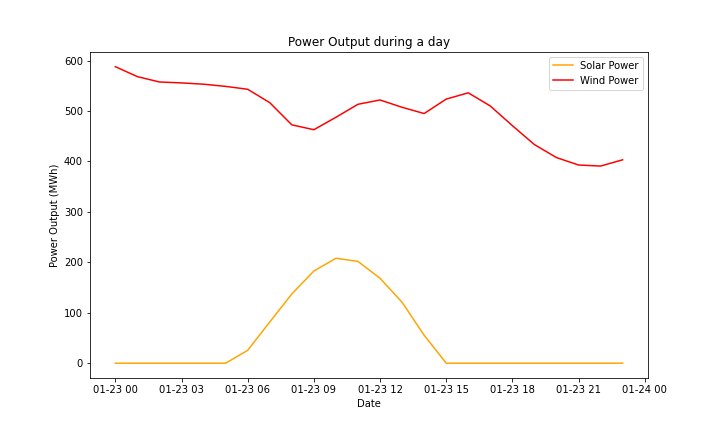
\includegraphics[width=\linewidth]{immagini/ImmaginiOptimization/balancedPowerOutputday.png}
%   \caption{Solar and Wind Power Output (MWh)}
%   \label{fig:balance day power}
% \end{subfigure}%
% \begin{subfigure}{.5\textwidth}
%   \centering
%   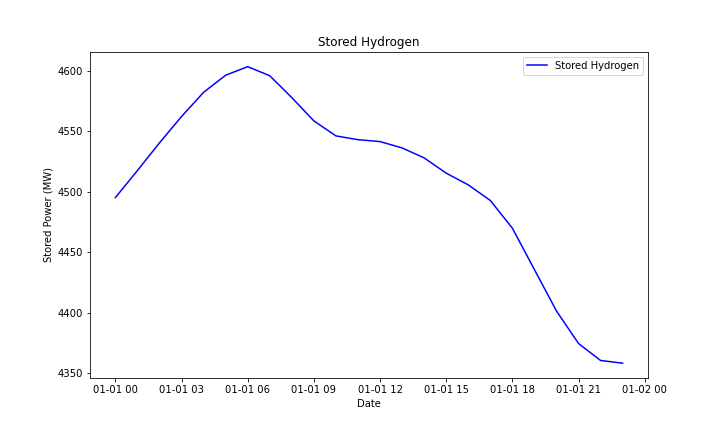
\includegraphics[width=\linewidth]{immagini/ImmaginiOptimization/balanceHH1day.png}
%   \caption{ Hydrogen Storage (MW)}
%   \label{fig:balanced day hydrogen}
% \end{subfigure}
% \caption{Power Production in one day}
% \label{fig:balanced day}
% \end{figure}


%provo a fare a 3 scenari invece che 5
%ma quando metto il upper bound dell'eolico sopra i 350 ci mette una vita
%solo che l'ottimo sta intorno ai 540
% grrrr miao
%ti faccio sapere

% Heyyyyyyy <3 <3<3<3
%miao miao
%ce manca
%Non so forse metterei prima il modello determinisco che di fatti è il focus principale.
% Cioè il fatto che ci siano degli scenari è abbastanza standard, anche se non spieghi subito da dove vengono.
%Questa parte vorrei poi scrivere meglio cosa è fatto nel codice ecc ecc come hai fatto te nella prim parte ma posso farlo io :)
%Te puoi concentrarti su i Results subsection
% A certo il classico tempo di risoluzione che dipende dall'umore del computer. Grande classico ahahah LOL
%MHHH strano



\newpage
\printbibliography[
heading=bibintoc,
title={Bibliography}]





%\end{justify}





\end{document}
